% Reviewer 2 responses

\begin{point}
The ``General-Purpose Models for the Chemical Sciences'' review by Alampara et al. is an extraordinarily ambitious summary (well over 170 pages) that seeks to chart the landscape of foundation-style AI models in chemistry. The authors have gathered an impressive amount of literature, most of which not related to the objective of the review.
\end{point}

\begin{reply}
\label{reply:depth_breadth}
We thank the reviewer for acknowledging the ambition of our work. We have now extensively reviewed and pruned the references we cite, removing 50+ citations that were not directly relevant to \glspl{gpm}. In particular, we also revised all sections in the application part to emphasize depth over breadth. For instance, in the section about property prediction, we now discuss fewer examples in the main text and moved many references to a comparative table. 
\end{reply}

\begin{point}
The manuscript is currently too dispersive, diffuse and uneven to meet Chemical Reviews standards. A sharper focus on genuine general-purpose (foundation) models, tighter organization, and a more consistently critical voice will be needed before the article can be recommended for publication in this venue. For these reasons, I recommend a major revision (borderline).
\end{point}

\begin{reply}
\label{reply:diffuse}
 We have now:
\begin{itemize}
\item Reviewed Sections 5, 6, and 7, making them more focused, discussing only works that add significant value to the topic.
\item Provided a more critical voice by adding explicit ``Limitations'' and ``Open Challenges'' subsections for all applications discussed in Sections 5 and 6.
\item We also now integrated \enquote{example boxes} throughout Section 3, which walks through key concepts with chemistry-specific examples. (See our response \Cref{reply:example_boxes})
\item Sharpened our focus on genuine \glspl{gpm} by adding a clear definition and comparison table (Table 1) early in the manuscript. (See our response to reviewer 1 \Cref{reply:gpm_definition})
\end{itemize}
\end{reply}

\begin{point}
The review introduces ``general-purpose models'' (GPMs), such as LLM, and then surveys literally everything from data formats and model architectures to molecule design, retrosynthesis, education, and ethics. That goes well beyond the objective stated in the abstract and missing the Chemical Reviews standards. The manuscript is overly ambitious in aiming to be a one-stop resource for how AI might transform every stage of chemical research, rather than focusing on GPMs.
\end{point}

\begin{reply}
\label{reply:prune}
We have now reviewed the entire article, where we very early in the paper define \glspl{gpms} and distinguish them from other types of models. See our response \Cref{reply:gpm_definition}, where we introduce a new table and definition.

Apart from that, we have now extensively pruned different sections as mentioned in responses \Cref{reply:diffuse} and \Cref{reply:depth_breadth}.
For example, in the materials generation and property prediction section, we removed all the enumeration of incremental work and moved citations to a table (see \Cref{tab:property_prediction_models}). Apart from incremental works, we also pruned tangential discussions. For example, in experiment execution, we removed discussions related to protocol languages.

\begin{table}[htbp]
    \centering
    \caption{\textbf{Non-comprehensive list of \glspl{gpm} applied to property prediction tasks}. The table presents different models and their applications across different molecular and materials property prediction benchmarks, showing the diversity of properties (from molecular toxicology to crystal band gaps), datasets used for evaluation, modeling approaches (prompting, fine-tuning, or retrieval-augmented generation), and task types (classification or regression.)}
    \label{tab:property_prediction_models}
    \resizebox{\textwidth}{!}{%
    \begin{tabular}{lllcc}
        \toprule
        \textbf{Model} & \textbf{Property} & \textbf{Dataset} & \textbf{Approach}  & \textbf{Task}\\
        \cmidrule{1-5}
        \multirow{3}{*}{LLM-Prop\autocite{rubungo_llm-prop_2023}} & Band Gap & \multirow{3}{*}{CrystalFeatures-MP2022\autocite{rubungo_llm-prop_2023}} & \multirow{3}{*}{P} &  R  \\
        & Volume & & & R \\
        & Band gap &  & & C \\
        \midrule
        \multirow{12}{*}{LLM4SD\autocite{zheng2025large}} & Blood-brain barrier penetration & BBBP\autocite{sakiyama_prediction_2021} & \multirow{10}{*}{P} & C \\
        & FDA approval & ClinTox\autocite{wu2018moleculenet} & & C \\
        & Toxicology & Tox21\autocite{richard_tox21_2021} & & C \\
        & Drug-related side effects & SIDER\autocite{kuhn_sider_2016} & & C \\
        & HIV replication inhibition & HIV\autocite{wu2018moleculenet} & & C \\
        & $\beta$-secretase binding & BACE\autocite{wu2018moleculenet} & & C \\
        & Solubility & ESOL\autocite{wu2018moleculenet} & & R \\
        & Hydration Free Energy & FreeSolv\autocite{mobley_freesolv_2014} & & R \\
        & Lipophilicity & Lipophilicity\autocite{wu2018moleculenet} & & R \\
        & Quantum Mechanics & QM9\autocite{wu2018moleculenet} & & R \\
        \midrule
        \multirow{3}{*}{Domain Knowledge Prompt-Engineering\autocite{liu2025integrating}} & Crystal & Custom\autocite{liu2025integrating}& \multirow{3}{*}{P}   &\multirow{3}{*}{C,R}\\
        & Organic Small Molecules & PubChem\\
        & Enzymes & UniProt\\
        \midrule
        \multirow{10}{*}{MolecularGPT\autocite{liu2024moleculargpt}} & $\beta$-secretase binding & BACE \autocite{wu2018moleculenet} & \multirow{10}{*}{P} & C\\
        & HIV replication inhibition & HIV\autocite{wu2018moleculenet} & & C\\
        & Bioactivity & MUV \autocite{rohrer2009maximum} & & C\\
        & Toxicology & Tox21 \autocite{richard_tox21_2021} & & C \\
        & Toxicology & ToxCast \autocite{us2015toxicity} & & C\\
        & Blood-brain barrier penetration & BBBP\autocite{sakiyama_prediction_2021} & & C\\
        & Cytochrome P450 isozymes & CYP450 \autocite{ni2025curated} & & C\\
        & Solubility & ESOL \autocite{delaneyesol2004} & & R\\
        & Hydration Free Energy & FreeSolv \autocite{mobley_freesolv_2014}& & R\\
        & Lipophilicity& Lipophilicity\autocite{wu2018moleculenet} & & R\\
        \midrule
        \multirow{9}{*}{GPT-MolBERTa \autocite{balaji2023gptmolberta}} & Blood brain barrier penetration & BBBP\autocite{sakiyama_prediction_2021} & \multirow{9}{*}{P} & C\\
        & Toxicity & Tox21 \autocite{richard_tox21_2021} & & C\\
        & Toxicity & Toxcast \autocite{us2015toxicity} & & C\\
        & FDA Approval & Clintox \autocite{wu2018moleculenet} & & C \\
        & Solubility & ESOL \autocite{delaneyesol2004} & & R\\
        & Hydration Free Energy& FreeSolv\autocite{mobley_freesolv_2014} & &R \\
        & Lipophilicity & Lipophilicity \autocite{wu2018moleculenet}& & R\\
        & HIV replication inhibition& HIV\autocite{wu2018moleculenet} & & C\\
        &  $\beta$-secretase binding & BACE \autocite{wu2018moleculenet} & &  C\\
        \midrule
        \multirow{7}{*}{GPT-Chem\autocite{jablonka2024leveraging}} & HOMO/LUMO & QMUGs\autocite{isert_qmugs_2022} & \multirow{7}{*}{FT} & C, R \\
        & Solubility & DLS-100\autocite{mitchell_dls-100_2017} & & C, R \\
        & Lipophilicity & LipoData\autocite{jablonka2024leveraging} & & C, R \\
        & Hydration Free Energy & FreeSolv\autocite{mobley_freesolv_2014} & & C, R \\
        & Photoconversion Efficiency & OPV\autocite{jablonka2024leveraging} & & C, R  \\
        & Toxicology & Tox21\autocite{richard_tox21_2021} & & C, R  \\
        & $\text{CO}_2$ Henry Coefficients of MOFs & MOFSorb-H\autocite{lin_silico_2012} & & C, R \\        
        \midrule
        \multirow{4}{*}{\modelname{LLaMP\autocite{chiang2024llamp}}} & Bulk modulus & \multirow{4}{*}{Materials Project\autocite{riebesell2025framework}} & \multirow{4}{*}{RAG} & R \\
        & Formation energy & & & R \\
        & Electronic bandgap & & & R \\
        & Multi-element electronic bandgap & & & R \\
        \bottomrule
    \end{tabular}
    }
    \vspace{0.5em}
    \footnotesize
    \begin{minipage}{\linewidth}
        \textbf{Key:}  P = prompting; FT = fine-tuned model; RAG = retrieval-augmented generation; C = Classification; R = Regression
    \end{minipage}
\end{table}


% Also to make the rationale behind discussing a breadth of application clearer, we added the following to at the beginning of the applications section:
% \begin{quote}
% True acceleration of chemical research and the ultimate goal of fully autonomous science require AI systems that can operate across the entire scientific workflow. The stages outlined in Section 5.1.5—from hypothesis generation to experimental execution and final reporting—represent the core of this process. While GPMs, especially LLMs, show promise in individual components, for AI to evolve from a useful tool into a driver of fully autonomous research, it must therefore master the entire workflow, seamlessly navigating between each of these crucial stages.
% \end{quote}

With the new changes, we now do not aim to review all existing approaches for a given application but rather show how \glspl{gpm} have and could be used for various applications.

\end{reply}

\begin{point}
The stated focus is GPMs, yet much of the text drifts into robotics, classic QSAR, and other areas only tangentially related to foundation models/GPMs. Removing these digressions would help readers see the wood for the trees. This would also serve in removing a large number of references that nothing have to do with GPMs, or even with AI (see a series of related to the Chemputer by Cronin - many other examples beyond this are present). Rather than a review on GPMs seems more a textbook on Digital Chemistry. Authors must perform some heavy clean-up and refocusing around the main objective of the work.
\end{point}

\begin{reply}

As discussed in response to \cref{reply:prune}, we streamlined the discussion.
In particular, we have made the experimental execution section more concise by removing references and discussions that diverged from \glspl{gpm}. We removed approximately 7 references related to the Chemputer and similar topics (\autocite{steiner2019organic}, \autocite{hammer2021chemputation}, \autocite{rauschen2024universal}, \autocite{strieth-kalthoff2024delocalized}, \autocite{wilbraham2021chemPU}, \autocite{mehr2023digitizing}, \autocite{leonov2024integrated})


\end{reply}

\begin{point}
Several recent reviews and perspectives (e.g. https://doi.org/10.1039/D4SC03921A; https://doi.org/10.1021/jacsau.4c01160 and others) cover similar ground. Please articulate, early and explicitly, what new perspective this article provides. A distinctive taxonomy, unified framework, or meta-analysis of model performance could do the job.
\end{point}

\begin{reply}
Our review provides several distinctive contributions that differentiate it from recent reviews:

\begin{itemize}
\item We introduce a clear taxonomy distinguishing \glspl{gpm} from domain-specific foundation models and specialized chemistry pipelines (see  \Cref{reply:gpm_definition}), with concrete examples and characteristic features for each category
\item We provide a unified framework that integrates the entire scientific workflow---from data collection to hypothesis generation, experimental planning, execution, and reporting.
\item We include critical ``Limitations'' and ``Open Challenges'' subsections for each application area, providing concrete failure cases and explicit discussion of when \glspl{gpm} should and should not be used. Apart from this, we have a quantitative meta-analysis of model performance across different tasks, including comparative error distributions showing where \glspl{llm} underperform specialized models in property prediction tasks in the application section. (See for example \Cref{fig:property_limitations} below)
\item We incorporated worked-out examples into our figures (see, for example, \Cref{fig:planning})
\item We provide substantially deeper technical coverage of fundamental building principles and design of evaluations  (Sections 2-4) compared to existing reviews. Based on the recommendations from the reviewers, we have now also included chemistry-specific examples throughout the section. (see for example \Cref{example:multimodal})
\end{itemize}

\begin{figure}[H]
    \centering
    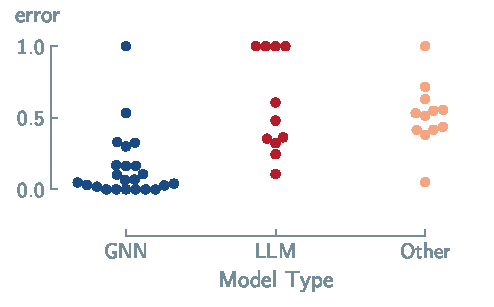
\includegraphics{figures/property_mattext.pdf}
    \caption{\textbf{Normalized error distributions for materials property prediction models across different architectures}. Each point represents the normalized error of a model on a specific property prediction task. Normalization was achieved with min/max values of each dataset to produce a range of errors between 0 and 1. The first column (blue) shows \gls{gnn} based models, the second column (red) displays \gls{llm} approaches, and the third column (orange) represents other baseline methods and \gls{sota} models, including \modelname{CrabNet}. \autocite{Wang_2021} Lower values indicate better predictive performance.}
    \label{fig:property_limitations}
\end{figure}



\begin{figure}[!htbp]
    \centering
        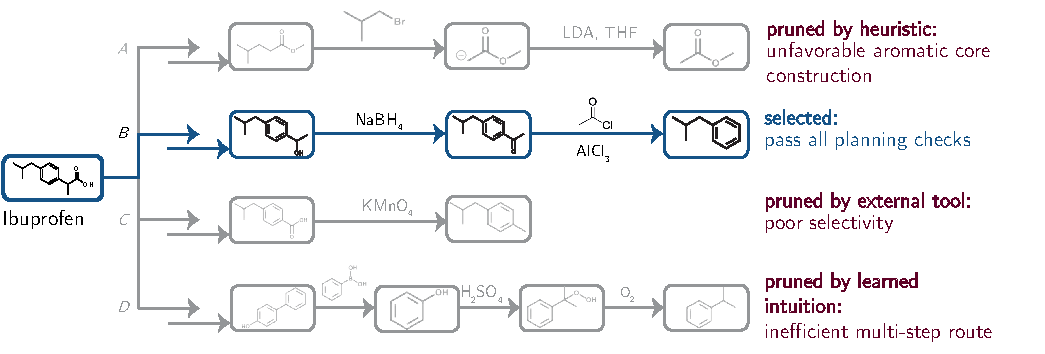
\includegraphics[width=1\textwidth]{figures/rescaled_figures/chemrev_figure14.pdf}
    \caption{\textbf{\gls{gpm}-guided retrosynthesis route planning and pruning}. \glspl{gpm} can systematically evaluate and prune retrosynthetic routes using multiple reasoning capabilities to discriminate between viable and problematic approaches. The partially overlapping arrows at the start of each route indicate multiple steps. \textbf{Route A}: This route was pruned by heuristic reasoning due to the unfavorable aromatic core construction.
    \textbf{Route B}: This route was selected as it successfully passes all \gls{gpm} planning checks, demonstrating optimal synthetic feasibility.
    \textbf{Route C}: This pathway was pruned by external tools due to the poor regio-selectivity of the oxidation step.
    \textbf{Route D}: This route was pruned based on learned intuition, as it represents an inefficient multistep pathway; the route could just start with phenol instead of synthesizing it.
}
    \label{fig:planning}
\end{figure}

\begin{examplebox}[label={example:multimodal}]{Multimodal reasoning for chemical identification}
A chemist finds an unknown white powder in a food sample which is highly soluble in water and tastes sweet. Chemist wants to identify it: \\
\textbf{Input Modalities:}
\begin{itemize}
    \item \textbf{$^{13}$C-NMR spectrum:} Shows peaks in the 60--100 ppm region, characteristic of carbons bonded to oxygen.
    
    \item \textbf{$^{1}$H-NMR spectrum:} Multiple peaks in the 3--5 ppm region with complex splitting patterns, indicating protons on oxygen-bearing carbons.
    
    \item \textbf{IR spectrum:} Broad, intense peak at 3000--3500 cm$^{-1}$ (O-H stretching), peaks around 2900 cm$^{-1}$ (C-H stretching), strong peaks at 1000--1150 cm$^{-1}$ (C-O stretching, ether and alcohol).
    
    \item \textbf{Mass spectrometry:} Molecular ion peak at \texttt{m/z = 180}.
    
    \item \textbf{Text description:} \enquote{White crystalline solid, sweet taste, highly soluble in water, found in food sample}.
    
\end{itemize}
\textbf{Multimodal Model Reasoning:}
\begin{itemize}
    \item \textbf{MS + IR $\rightarrow$} Molecular formula \ce{C6H12O6} with multiple hydroxyl groups (polyol).
    \item \textbf{NMR $\rightarrow$} Chemical shifts and splitting patterns consistent with a cyclic structure containing multiple oxygen-bearing carbons; presence of anomeric signals suggests equilibrium between ring forms.
    \item \textbf{Text + Chemical Knowledge $\rightarrow$} Sweet taste and high water solubility point to a simple sugar (monosaccharide).
\end{itemize}
Based on the evidence, the model hypothesizes the molecule to be D-glucose. Single modality would be insufficient---mass spectrometry alone could match any hexose isomer (fructose, galactose, etc.), but combining spectroscopic fingerprints with physical properties enables confident identification.
\end{examplebox}

We now write at the end of introduction,

\begin{quote}
    We hope to contribute to this by addressing chemists and computer scientists, by providing technical background, a consistent terminology, and explaining key technical terminology in a glossary at the end of the manuscript.
\end{quote}
\end{reply}

\begin{point}
Many subsections read like annotated bibliographies. I would rather see fewer examples examined in greater depth (why they succeed, where they fail, and what they teach us) than exhaustive tallies of every preprint. Authors need to address this point.
\end{point}

\begin{reply}
We have addressed this concern by substantially editing the applications sections (Sections 5-7). 
See our response to \Cref{reply:prune}
\end{reply}

\begin{point}
The tone often feels boosterish. Each technical section should balance accomplishments with known limitations (hallucination rates, failure modes in retrosynthesis, domain-shift issues, data leakage, etc). The more candid you are, the more valuable the review becomes. Authors need to address this point.
\end{point}

\begin{reply}
We have made substantial changes to provide a more balanced and candid tone. Specifically:

We added explicit ``Limitations'' subsections in each application section discussing known failure modes, hallucination issues, domain-shift problems, data leakage concerns, and other critical limitations.
See, for example, an excerpt from the \glspl{gpm} as optimizers section on limitations and open challenges:

\begin{quote}
    
\paragraph{Limitations}
Current \glspl{llm} for chemical optimization, to date, exhibit a pronounced volatility, rarely yielding stable performance gains. 
Their outcomes are highly sensitive to prompt phrasing, and a lack of calibrated uncertainty estimates prevents their use for principled acquisition strategies. \autocite{liu2024large}
Furthermore, these models frequently produce hallucinations and violate critical constraints, leading to invalid chemical structures or the proposal of unsafe and infeasible experimental conditions. 
Alleged improvements often hinge on narrow benchmarks, extensive pre- and post-processing, or access to downstream oracles, rather than on robust chemical reasoning. 
Within hybrid pipelines, the specific contribution of the \gls{llm} becomes difficult to isolate.

\paragraph{Open Challenges}
\begin{itemize}
    \item \textbf{Correct Prompt Sensitivity}: A key challenge is achieving prompt invariance, where the ranking of candidates remains stable under controlled rephrasings. Promising research directions include developing rigorous invariance tests and moving beyond discrete tokens to leverage models' more stable hidden states \autocite{rankovic2025gollum0}.
    \item \textbf{More robust evaluations}: Future work should develop more robust frameworks that assess oracle realism, conduct thorough leakage audits to detect data contamination, and integrate uncertainty-aware metrics to better quantify risk and reliability.
    \item \textbf{Ablations for the specific LLM role}: There is a critical need for systematic ablation studies that isolate core \gls{llm} performance from enhancements like \gls{rag}, external scorers, or tool use. Such studies are essential for fairly comparing general and fine-tuned \glspl{llm} and for understanding the source of performance gains.
\end{itemize}
\end{quote}
\end{reply}

\begin{point}
Self-citations dominate several sections. Cite your own work where it is genuinely seminal, of course, but be sure to give equal weight to other leading groups. This is a critical requirement of Chemical Reviews. Also reconsider whether every arXiv preprint needs to be included. The current selection of works is unreasonable and most important, unjustified by the objectives of the review.
\end{point}

\begin{reply}
We have carefully reviewed our citations and made the following changes:
\begin{itemize}
\item Reduced citations to only those that are directly relevant and provide important contributions (removed more than 50+ citations overall).
\item Applied stricter criteria for inclusion, asking whether each cited work adds substantive value to understanding \glspl{gpm} in chemistry. We moved many incremental contributions from the main text to summary tables or removed them entirely if they did not add significant insights.
(See \Cref{tab:property_prediction_models}, Table 8 and the property prediction section)
\end{itemize}

\end{reply}

\begin{point}
Define ``GPM'' crisply and stick to it. Make clear whether it is synonymous with ``foundation model,'' whether multimodal models qualify, and so on. Harmonise acronyms across sections.
\end{point}

\begin{reply}
We have now added a crisp definition of GPM in Section 1 (Introduction) and stick to it throughout the manuscript:
\begin{quote}
A \gls{gpm} is a model that has been pre‑trained on a broad, heterogeneous corpus spanning multiple data modalities (text, images, graphs) or representations (e.g., common names, 3D coordinates, molecular images).
It can be applied to a wide spectrum of downstream tasks that differ in objective (classification, regression, generation, reasoning), input format, and domain---ranging from natural‑language processing to chemistry and vision---with little or no task‑specific fine‑tuning.
A \gls{gpm} supports zero‑shot, few‑shot, or transfer learning and can serve as the core component of autonomous agents.
\end{quote}

We also added Table 1 (see \Cref{tab:gpm}) to clarify the distinction between \glspl{gpm}, domain-specific foundation models, and specialized chemistry pipelines, with representative examples for each category. We explicitly explain that we adopt the term \gls{gpm} to avoid semantic overlap with ``foundation model'' and to signal the breadth of applicability. Multimodal models are included as a subcategory of \glspl{gpm}. We have harmonized acronym usage throughout all sections to maintain consistency.
\end{reply}

\begin{point}
Remove informal flourishes (e.g. the heart icon in the author list) and proof-read carefully, working on the entire manuscript with highest level of professionalism. There are encoding glitches (``flexibilit{\'y}'') and scattered typos.
\end{point}

\begin{reply}
We have now removed informal flourishes, including the heart icon in the author list, and reviewed the entire manuscript. We have specifically:
\begin{itemize}
\item Removed all non-standard icons and informal elements.
\item Carefully proofread the entire manuscript, ensuring consistent formatting throughout.
\end{itemize}
\end{reply}

\begin{point}
It could be even better if it proposed a short list of concrete, open research problems. In its current form, the review (through this section) does not address insights about the remaining challenges and future directions for the field. This is a critically important component of reviews that the author have to address substantially better.
\end{point}

\begin{reply}
This feedback led us to add ``Open Challenges'' subsections in each of the application sections (Sections 5 and 6) and the evaluation best practices box.
For example, see the open challenges in the experiment execution section and the molecular and material generation section,

\begin{quote}
    
\begin{itemize}
\item \textbf{Grounding Natural Language to Laboratory Actions.} Translating ambiguous natural-language instructions (\enquote{heat gently}) into precise, safe operations requires developing validation layers that detect physically impossible or hazardous actions before hardware execution.

\item \textbf{Universal Protocol Standards.} No widely adopted formalization standard exists. While languages like \gls{chidl} show promise, achieving interoperability across platforms requires community consensus on abstraction levels and device interfaces. \Glspl{mcp} offer a potential path forward by enforcing consistent interfaces between \glspl{gpm}, instruments, and verification layers.

\item \textbf{Autonomous Error Recovery.} Current systems cannot autonomously diagnose and recover from experimental failures. Developing general-purpose failure detection mechanisms and recovery strategies would enable truly autonomous operation.

\item \textbf{Multimodal Integration.} Chemists use diverse data types---spectra, chromatograms, TLC plates, and microscopy images. Integrating these modalities into \gls{gpm} decision-making loops remains technically challenging but essential for human-level experimental reasoning.

\item \textbf{Verification and Provenance.} Industrial and clinical applications require complete experimental provenance: every decision logged with reasoning traces, all parameters recorded, and outcomes traceable to specific model versions.
\end{itemize}
\end{quote}


\begin{quote}
    
\begin{itemize}
    \item \textbf{Robust Conditional Generation} Developing models that can reliably generate novel diverse structures that satisfy complex, multi-objective constraints (e.g., high stability, specific electronic properties, and synthesizability) without over-relying on retrieved training data examples.
    \item \textbf{Bridging the Synthesis Gap} Creating new validation metrics that better predict the synthetic feasibility of generated materials and molecules, moving beyond structural similarity toward realistic pathway prediction
    \item \textbf{Unified Multi-Scale Generation} Developing frameworks that are capable of simultaneously modeling different representations (e.g., text, graphs, 3D structures) and scales (e.g., from non-planar molecules to crystalline materials) within a single generative process
 \end{itemize}
 \end{quote}
 
Similarly, we added explicit ``Limitations'' subsections pointing out more fundamental open questions.
\end{reply}

\shortpoint{Most schematic figures are dense. Simplify captions and ensure that all symbols are defined.}

\shortreply{We have revised the figures to improve clarity by simplifying figure captions to be more concise and focused, adding a glossary of symbols used in figures, reviewing figures to remove content that did not add value (e.g., removed Figure 23 from Section 7.1), and ensuring all symbols and notation are clearly defined either in the figure itself or in the caption.}

\shortpoint{Check every entry against ACS format and weed out duplicates or uncited items.}

\shortreply{ We have now checked all reference entries against ACS format requirements, removed duplicate entries and uncited items from the bibliography, and ensured all citations include complete information (authors, titles, journal names, years, volumes, and page numbers).}

\shortpoint{Consider whether ML background material that is not chemistry-specific can be shortened or moved online. This is a review, not a textbook for teaching classes.}

\shortreply{One distinguishing feature of our review is that we attempt to provide a unified perspective that highlights that the principles underlying \glspl{llm} can also be applied to other model architectures and datasets. We made this clearer with revisions to the introduction.
To make it even more accessible for a chemistry audience, we added chemistry-specific examples (see \Cref{reply:example_boxes}).}